\documentclass{beamer}
\usetheme{Madrid}

\usepackage{tikz}

\title{ML4AAD - Final Project}
\subtitle{Winter Semeseter 18/19}
\author{Neeratyoy Mallik}
\institute{4774378}
\date{\today}

\begin{document}
	
\begin{frame}
\titlepage
\end{frame}

%%
% SLIDE 1 - MOTIVATION
%%
\begin{frame}
\frametitle{Motivation (The Why)}
\begin{center}
\begin{tikzpicture}
	\onslide<1-4> \node (img1) {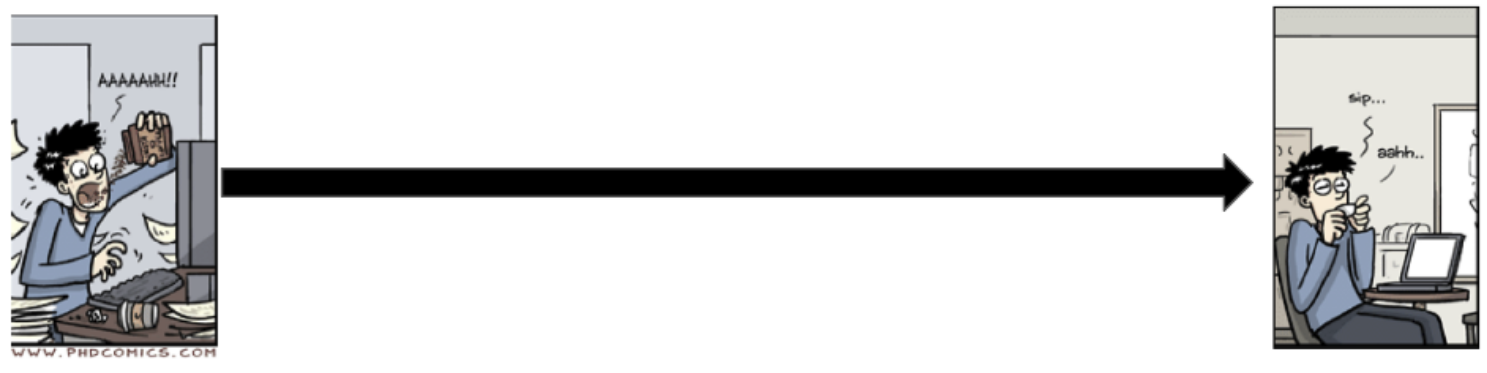
\includegraphics[scale=0.18]{../plots/motivation.png}};
	\pause
	\onslide<2> \node (img2) at (img1.south) {
\includegraphics[scale=0.18]{../plots/red_arrow.png}};
	\pause
\end{tikzpicture}
\end{center}
\begin{columns}
	\column{0.5\textwidth}
	\onslide<3-4> {2 Datasets with differing size, \# of classes, class balance}		\onslide<3-4>{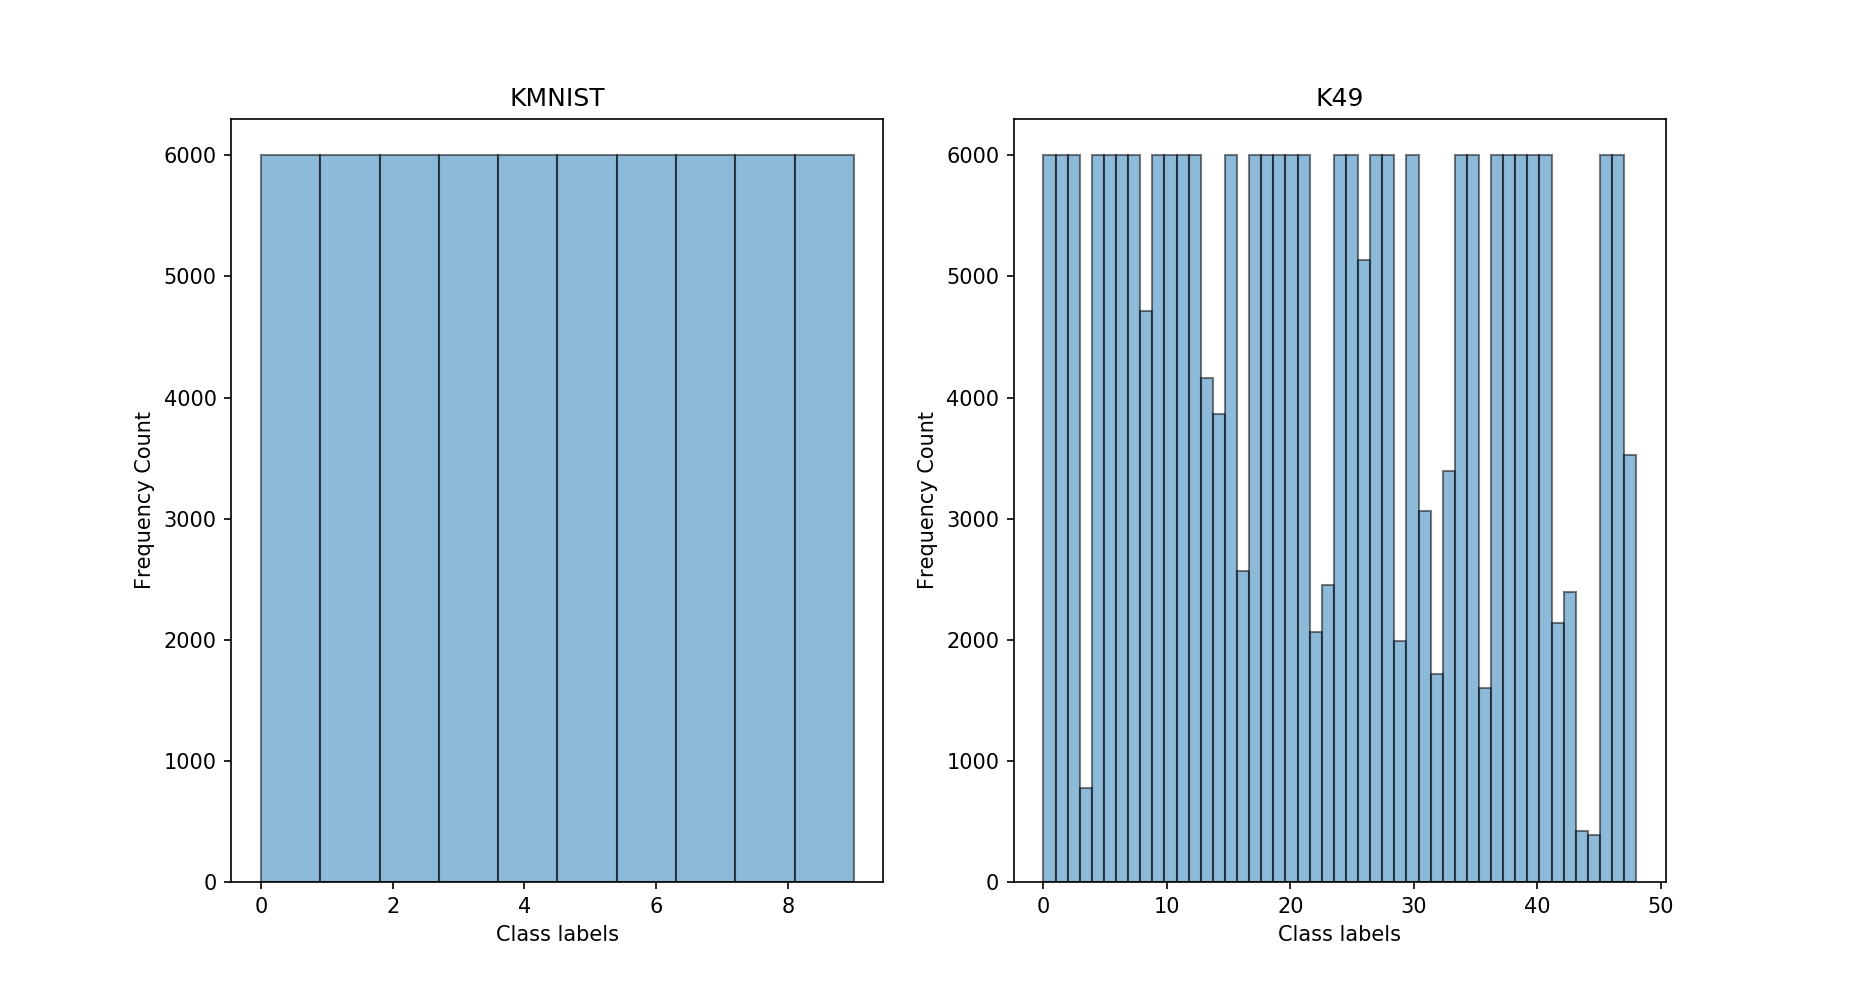
\includegraphics[scale=0.18]{../plots/class_distro_plot.png}}
	\pause
	\column{0.5\textwidth}
	\onslide<4> {BOHB outperforms SMAC in high dimensional, mixed data}
	\onslide<4> {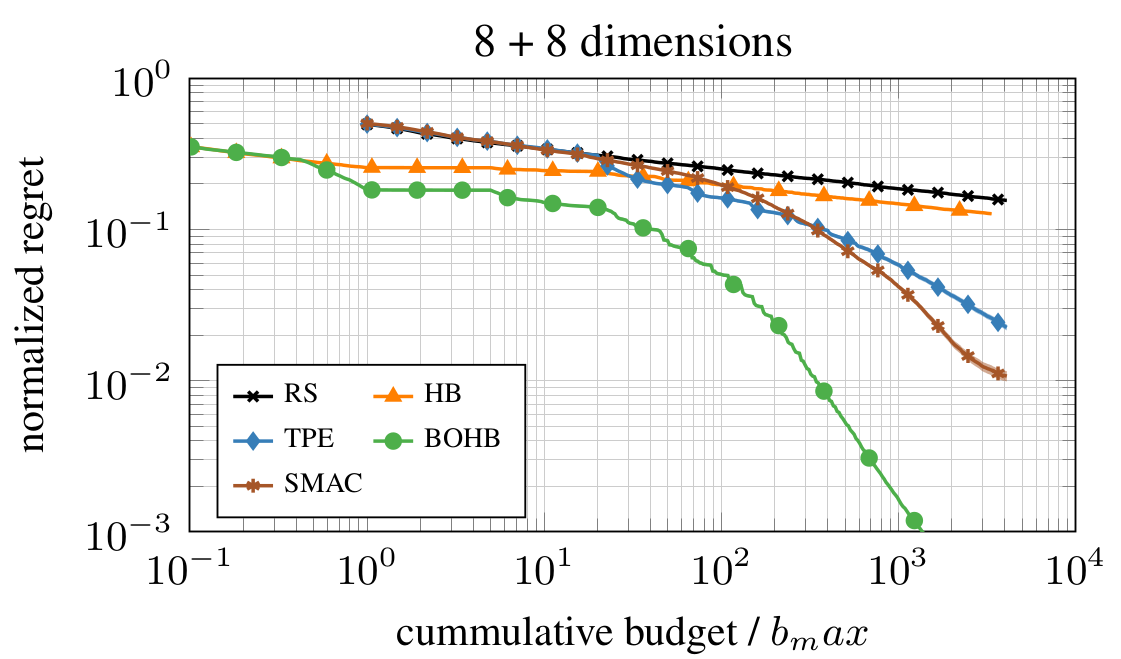
\includegraphics[scale=0.13]{../plots/bohb_smac.png}}
\end{columns}
\end{frame}


%%
% SLIDE 1 - BOHB and SETUP
%%
\begin{frame}
\frametitle{Design Decisions (and BOHB)}
CNN equation.
\end{frame}

\begin{frame}
\frametitle{KMNIST and K49}
Runs and results.
\end{frame}


\begin{frame}
\frametitle{The extra juice}
Data Augmentation.
\end{frame}


\begin{frame}
\frametitle{Final Results}
Final numbers to report.
\end{frame}

\end{document}